% Mindmap
% Author: Stefan Kottwitz
% https://www.packtpub.com/hardware-and-creative/latex-cookbook
\documentclass[border = 60pt]{article}
\usepackage[landscape]{geometry}
\usepackage{tikz}
\usetikzlibrary{mindmap}
\usepackage{metalogo}
% \usepackage{dtklogos}
\begin{document}
\begin{figure}
  \centering
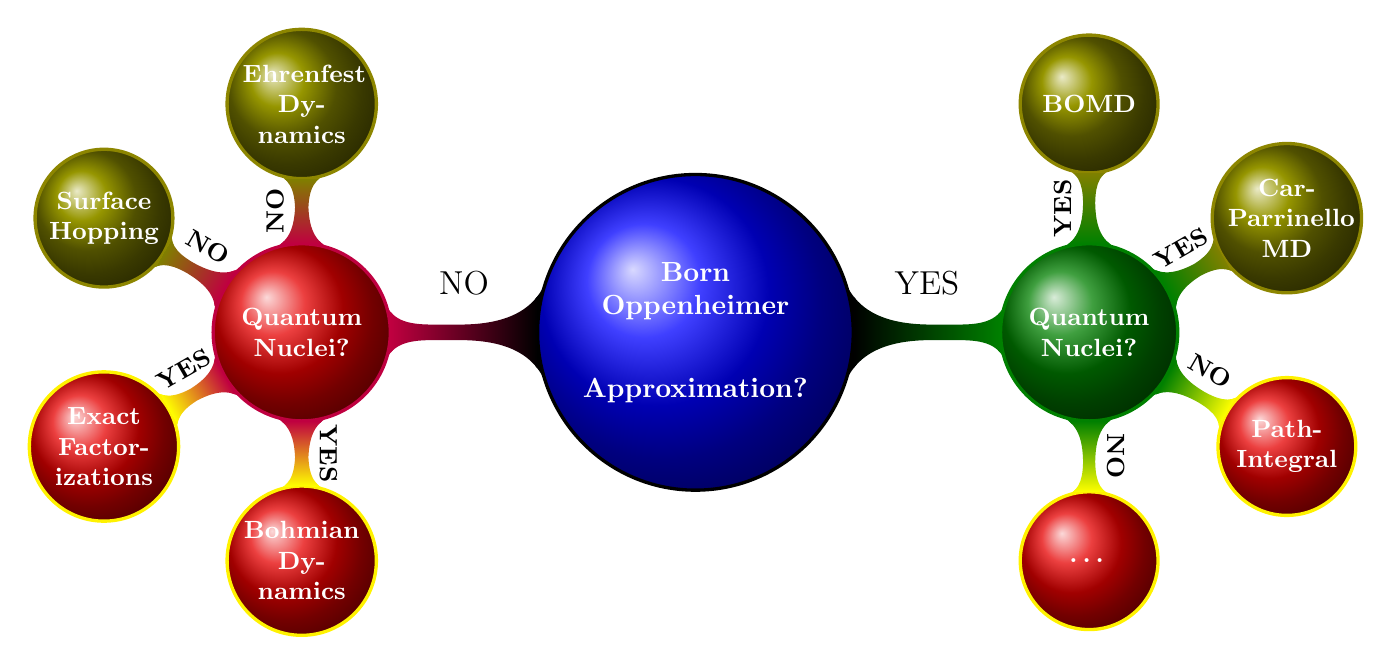
\begin{tikzpicture}
  \path [
    mindmap,
    text = white,
    % level 1 concept/.append style =
    %   {font=\Large\bfseries, sibling angle=60},
    level 2 concept/.append style =
      {font=\small\bfseries},
    level 3 concept/.append style =
      {font=\small\bfseries},
    root/.style= {
      concept, ball color=blue,
      font=\Huge\bfseries
    },
    BOY/.style = {concept, ball color=green!50!black},
    BON/.style = {concept, ball color=blue!50!black},
    QNY/.style = {concept, ball color=red!90!black},
    QNN/.style = {concept, ball color=olive!90!black}
  ]
  node (BOA) [root] {\normalsize Born\\ Oppenheimer\\ Approximation?} 
    child[concept color=green!50!black, nodes={BOY}, grow=0] {
      node (BOYES) {\small\bfseries Quantum Nuclei?}  [clockwise from=90]
        child [concept color=olive, nodes={QNN}] {
          node (bomd) {\small\bfseries BOMD}
        }
        child [concept color=olive, nodes={QNN}] {
          node (cpmd) {\small Car-Parrinello MD}
        }
        child [concept color=yellow, nodes={QNY}] {
          node (pimd) {\small Path-Integral}
        }
        child [concept color=yellow, nodes={QNY}] {
          node (etc)  {\small \ldots}
        }
      }
    child [concept color=purple, nodes={QNY}, grow=180] {
      node (BONO) {\small\bfseries Quantum Nuclei?} [counterclockwise from=90]
        {
          child [concept color=olive, nodes={QNN}] {
            node (EH) {\small Ehrenfest Dynamics}}
          child [concept color=olive, nodes={QNN}] {
            node (SH) {\small Surface Hopping}}
          child [concept color=yellow, nodes={QNY}] {
            node (EF) {\small Exact Factorizations}}
          child [concept color=yellow, nodes={QNY}] {
            node (BD) {\small Bohmian Dynamics}}
        }
      };
      
      \path (BOA)  --  node [anchor=south, yshift=10pt] {\large YES} (BOYES);
      \path (BOA)  --  node [anchor=south, yshift=10pt] {\large NO} (BONO);

      \path (BOYES)  --  node [align=center, sloped, above=3pt] {\small\bfseries YES} (bomd);
      \path (BOYES)  --  node [align=center, sloped, above=3pt] {\small\bfseries YES} (cpmd);
      \path (BOYES)  --  node [align=center, sloped, above=3pt] {\small\bfseries NO} (pimd);
      \path (BOYES)  --  node [align=center, sloped, above=3pt] {\small\bfseries NO} (etc);

      \path (BONO)  --  node [align=center, sloped, above=3pt] {\small\bfseries YES} (EF);
      \path (BONO)  --  node [align=center, sloped, above=3pt] {\small\bfseries YES} (BD);
      \path (BONO)  --  node [align=center, sloped, above=3pt] {\small\bfseries NO} (EH);
      \path (BONO)  --  node [align=center, sloped, above=3pt] {\small\bfseries NO} (SH);
\end{tikzpicture}
\end{figure}
\end{document}

%%% Local Variables:
%%% mode: latex
%%% TeX-master: t
%%% End:
